\section{Rauschen}

\subsection{Übersicht der Grössen und Zusammenhänge}

\begin{minipage}[c]{0.8\columnwidth}
    \renewcommand{\arraystretch}{1.5}
    \begin{tabular}{lll}
        $e_n$               & Rauschspannungsdichte                     & $[e_n] = \frac{\volt}{\sqrt{\hertz}}$ \\
        $v_n$               & Rauschspannung (\textbf{Effektivwert})    & $[v_n] = \volt$ \\
        $e_n^2$ (oder $S$)  & Rauschleistungsdichte                     & $[e_n^2] = \frac{\volt^2}{\hertz}$ \\
        $E$                 & Rauschleistung                            & $[E] = \volt^2$ \\
    \end{tabular}
    \renewcommand{\arraystretch}{1}
\end{minipage}
\hfill
\begin{minipage}[c]{0.18\columnwidth}
    $$ \boxed{ E = \int\limits_{0}^{\infty} e_n^2 \, \diff f } $$
    $$ \boxed{ E =  v_n^2 } $$
\end{minipage}

\vspace{0.2cm}
\textbf{Hinweis:} Ein guter Anhaltspunkt für die Zusammenhänge sind die Einheiten!


\subsection{Rauschen in der Elektronik}

\begin{outline}
    \1 \textbf{Alle Teile eines elektronischen Systems rauschen!}
    \1 Messpfad: Es sollen keine Störsignale zum Messsignal addiert werden
        \2 Ausser bei perfekter Abschirmung und Temperatur $0 \, \kelvin$ gibt es \textbf{immer} Störeinflüsse
\end{outline}

\begin{outline}
    \1 \textbf{ADC} und DAC: Quantisierungsrauschen $q$ (Quantisierungsschritt)
        \2 Quantisierungsrauschen (Auflösung) soll etwa so gross gewählt werden, wie das elektronische Rauschen
    \1 'Reine DC-Spannungen' gibt es nicht!
        \2 Auch DC-Signale haben Spannungs-Schwankungen
\end{outline}


\subsection{Arten von Rauschen}

\begin{minipage}[t]{0.48\columnwidth}
    \begin{itemize}
        \item \textbf{Thermisches Rauschen}
        \item \textbf{Flicker Noise} $\frac{1}{f}$-Noise
    \end{itemize}
\end{minipage}
\hfill
\begin{minipage}[t]{0.48\columnwidth}
    \begin{itemize}
        \item Shot Noise
        \item Burst (Popcorn) Noise
        \item Avalanche Noise
    \end{itemize}
\end{minipage}


\subsubsection{Thermisches Rauschen}

\begin{outline}
    \1 Entsteht durch \textbf{zufällige Bewegung der Ladungsträger} aufgrund der \textbf{Wärmeenergie}
        und der \textbf{Quantisierung der Ladung}
    \1 Ist über die Frequenzen \textbf{gleichverteilt}
    \1 Begriff: Weisses Rauschen
        \2 Anderer Ausdruck: Johnson Noise
\end{outline}


\subsubsection{Flicker Noise (Funkelrauschen)}

\begin{outline}
    \1 Entsteht am \textbf{Übergang} von zwei Materialien
        \2 u.a. in MOS-FET, wenn isch Elekronen in Fehlerstellen zw. Silizium und Gate-Oxid oder zw. Gate-Oxid 
            und Gate verfangen und nach gewissen Zeit zufällig wieder freikommen
    \1 Rauschleistung nimmt \textbf{umgekehrt proportional zur Frequenz ab} \textrightarrow\ $\frac{1}{f}$-Noise
    \1 Jede Dekade liefert die gleiche Rauschleistung
\end{outline}


\subsection{Amplitude und Leistung des Rauschens}

\textbf{Hinweis:} Als 'Leistung' gilt die \textbf{quadrierte Spannung}

\renewcommand{\arraystretch}{2}
\begin{tabular}{ll}
    Mittelwert der Rauschspannung               & $\overline{v_n}(t) = \frac{1}{T} \int_T v_n(t) \, \diff t \bm{= 0}$ \\
    Mittelwert der Rauschleistung (Varianz)     & $\overline{v_n(t)^2} = \overline{E} = \frac{1}{T} \int_T v_n^2(t) \, \diff t \bm{\neq 0}$ \\
    Effektivwert (Wurzel der Varianz)           & $\overline{v_{n, \rm rms}} = \sqrt{\overline{v_n(t)^2}} $\\
\end{tabular}
\renewcommand{\arraystretch}{1}


\subsubsection{Berechnung von Rauschen (!)}

\begin{outline}
    \1 Signale und Rauschen addieren sich \textbf{nicht gleich}
        \2 Deterministische \textbf{Signale}: \textbf{Amplituden} addieren sich
        \2 Stochastische Rauschquellen: \textbf{Rauschleistungen} addieren sich
\end{outline}


\subsection{Rauschen von Widerständen}

\begin{itemize}
    \item \textbf{Jeder Widerstand rauscht, unabhängig vom Stromfluss}
    \item Rauschen kann auf folgende zwei Arten modelliert werden
\end{itemize}

\begin{minipage}[c]{0.15\columnwidth}
    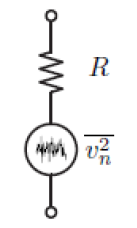
\includegraphics[width=\columnwidth]{images/rauschquelle_spannung.png}
\end{minipage}
\hfill
\begin{minipage}[c]{0.21\columnwidth}
    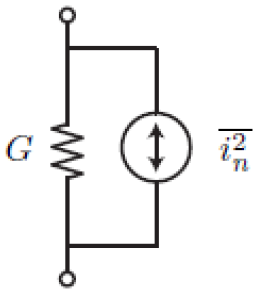
\includegraphics[width=\columnwidth]{images/rauschquelle_strom.png}
\end{minipage}
\hfill
\begin{minipage}[c]{0.62\columnwidth}
    \begin{minipage}[c]{0.48\columnwidth}
        $$ \boxed{ E = \overline{v_n^2} = 4 k T R B } $$
    \end{minipage}
    \hfill
    \begin{minipage}[c]{0.48\columnwidth}
        $$ \boxed{ E = \overline{i_n^2} = 4 k T G B } $$
    \end{minipage}
    \vspace{0.2cm}

    \begin{tabular}{l l c}
        $\overline{v_n^2}$  & mittlere Rauschleistung   & $[\overline{v_n^2}] = \volt^2$ \\
        $\overline{i_n^2}$  & mittlerer Rauschleistung  & $[\overline{i_n^2}] = \ampere^2$ \\ 
        $R$                 & Widerstand                & $[R] = \ohm$ \\
        $G$                 & Leitwert                  & $[G] = \siemens$ \\
        $B$                 & Bandbreite                & $[B] = \hertz$ \\
        $T$                 & absolute Temperatur       & $[T] = \kelvin$ \\
        \end{tabular}
        \begin{tabular}{ll}
        $k$                 & Boltzmann-Konstante $k = 1.38 \cdot 10^{-23} \, \frac{\joule}{\kelvin}$ \\
    \end{tabular}
\end{minipage}

$$ \boxed{ \text{Mittlere Rauschleistungsdichte (in)} \frac{\volt^2}{\hertz}:  4 k T R } $$ 


\subsubsection{Serieschaltung von Widerständen}

\begin{minipage}[c]{0.4\columnwidth}
    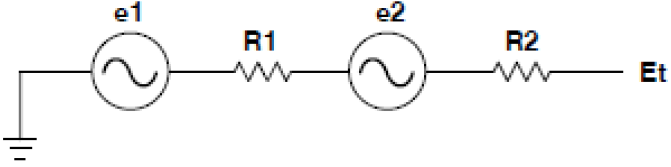
\includegraphics[width=\columnwidth]{images/serieschaltung_rauschende_widerstaende.png}
\end{minipage}
\hfill
\begin{minipage}[c]{0.58\columnwidth}
    \begin{minipage}[c]{0.48\columnwidth}
        $$ \boxed{ \overline{E_t^2} = \overline{e_1^2} + \overline{e_2^2} } $$
    \end{minipage}
    \hfill
    \begin{minipage}[c]{0.48\columnwidth}
        $$ [E_t] = [e_i^2] = \volt^2 $$
    \end{minipage}
\end{minipage}

\vspace{0.2cm}
\textbf{Nicht die Rauschspannungen, sondern die Rauschleistungen müssen addiert werden!} 


\subsection{Rauschen von Spannungsteilern}

\begin{minipage}[c]{0.13\columnwidth}
    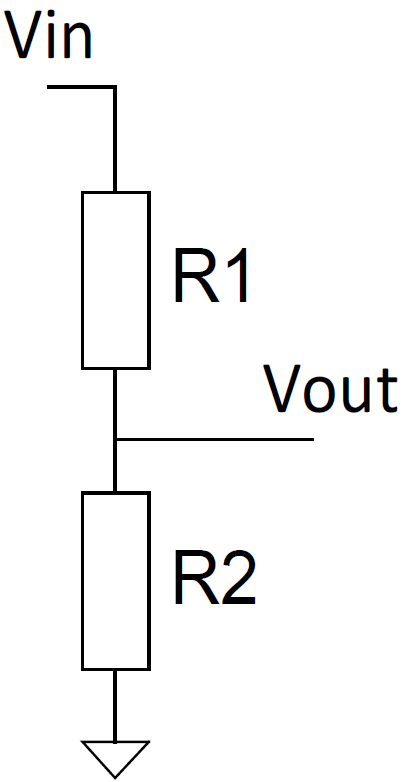
\includegraphics[width=\columnwidth]{images/rauschen_spannungsteiler.png}
\end{minipage}
\hfill
\begin{minipage}[c]{0.8\columnwidth}
    Rauschquellen sind \textbf{Kleinsignalquellen!} \textrightarrow\ $V_{\rm in} =$ GND
    $$ \boxed{\text{Rauschleistung:} \quad E_{\rm Vout} = 4 k T \cdot \frac{R_1 \cdot R_2}{R_1 + R_1} } $$
    $$ \boxed{\text{Rauschspannung:} \quad V_{\rm rausch} = \sqrt{E_{\rm Vout} } } $$
\end{minipage}


\subsection{Rauschen von Netzwerken}

\subsubsection{Widerstandsnetzwerke}

\textbf{Widerstands-Netzwerke rauschen gleich stark wie der äquivalente Ersatzwiderstand} 

\example{Rauschen von Widerstandsnetzwerk}

\begin{minipage}[c]{0.28\columnwidth}
    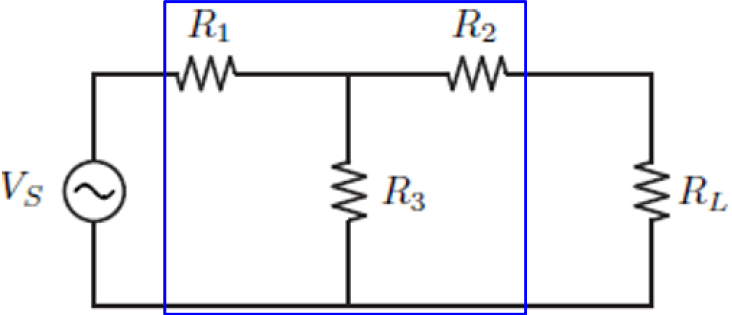
\includegraphics[width=\columnwidth]{images/gesamte_rauschspannung_schaltung.png}
\end{minipage}
\hfill
\begin{minipage}[c]{0.22\columnwidth}
    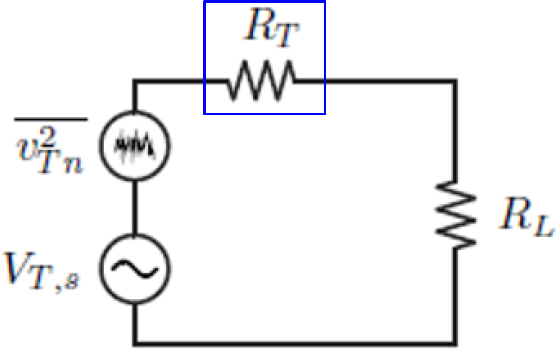
\includegraphics[width=\columnwidth]{images/gesamte_rauschspannung_ersatzschaltung.png}
\end{minipage}
\hfill
\begin{minipage}[c]{0.48\columnwidth}
    \renewcommand{\arraystretch}{1.4}
    \begin{tabular}{ll@{}}
        Ersatzwiderstand:   & $R_T = R_2 + R_1 || R_3$              \\
        Rauschleistung:     & $E = v^2_{Tn} = 4 k R_T B $           \\
        Rauschspannung:     & $v_{Tn} = \sqrt{v^2_{Tn}} = \sqrt{E}$ \\
    \end{tabular}
    \renewcommand{\arraystretch}{1}
\end{minipage}


\subsubsection{RC-Netzwerke}

\begin{itemize}
    \item Kapazitäten und Induktivitäten \textbf{rauschen nicht}!
    \item Kapazitäten und Induktivitäten beeinflussen die \textbf{Bandbreite} des Systems! \\
        \textbf{Rauschspannung indirekt beeinflusst}
\end{itemize}

\vspace{0.2cm}
\textrightarrow\ Sobald Kapazitäten oder Induktivitäten in einem Netzwerk vertreten sind, sind die Widerstände für das Rauschen egal!

\begin{minipage}[c]{0.28\columnwidth}
    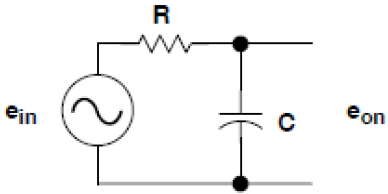
\includegraphics[width=\columnwidth]{images/rc_rauschen.png}
\end{minipage}
\hfill
\begin{minipage}[c]{0.7\columnwidth}
    $$ \boxed{ \text{Rauschspannung Ausgang:} \quad e_{\rm on} = \sqrt{\frac{k R }{C}} } $$
\end{minipage}


\example{Rauschen von RC-Netzwerken}    
    
Rauschspannungsdichte Widerstand: $e_{\rm in} = \sqrt{4 k T R}$
$$ e_{\rm on} = e_{\rm in} \sqrt{ \int\limits_{0}^{\infty} \frac{1}{1 + 2 \pi f R C} \, \diff f }
    = e_{\rm in} \sqrt{\frac{1}{1 + 2 \pi f R C} \Biggl[ \tan^{-1}\big( 2 \pi f R C \big) \Biggr]_{0}^{\infty} } 
    = e_{\rm in} \sqrt{\frac{1}{1 + 2 \pi R C} \frac{\pi}{2} } $$
Rauschspannung Ausgang: \quad $e_{\rm on} = \sqrt{4 k T R} \sqrt{\frac{1}{4 R C}} = \sqrt{\frac{k R }{C}} $


% \subsection{Vorgehen Gesamt-Rauschen berechnen}
% \label{Gesamt-Rauschen}

% \begin{itemize}
%     \item Lastwiderstände der Schaltung 'abhängen'
%     \item Spannungs- und Stromquellen 'ausschalten'
%     \item Von $R_L$ 'in Schaltung hineinschauen und Ersatzwiderstand $R_T$ berechnen
%     \item Rauschleistung und ev. Rauschspannung berechnen
% \end{itemize}


% \subsubsection{Tipps und Tricks} 

% \begin{outline}
%     \1 \textbf{Impedanzen}(Kondensatoren, Spulen)
%         \2 Rausch\textbf{leistung} berechnen (per Integral, da Impendanz variabel in Frequenz)
%     \1 \textbf{Parallelschaltung} von Widerständen / Impedanzen
%         \2 Rauschleistungen der einzelnen Komponenten separat berechnen
%         \2 Einzelne Rauschleistungen \textbf{addieren}
%         \2 Falls Rauschspannung gesucht: Wunzel ziehen 
% \end{outline}


\subsection{Rauschbandbreite}

\begin{itemize}
    \item In Realität werden Signal und Rauschen Tiefpass-gefiltert
    \item \textbf{Rauschbandbreite nicht identisch mit $\bm{3 \, \deci \bel}$-Bandbreite!} \\
        \textrightarrow\ ENB (Effective Noise Bandwidth)
\end{itemize}

\vspace{0.2cm}
Für $n$ kaskadierte Butterworth-Filter 1. Ordnung mir Grenzfrequenz $f_c = \frac{1}{2 \pi R C}$ verhält sich das ENB gemäss:

\begin{minipage}[c]{0.6\columnwidth}
    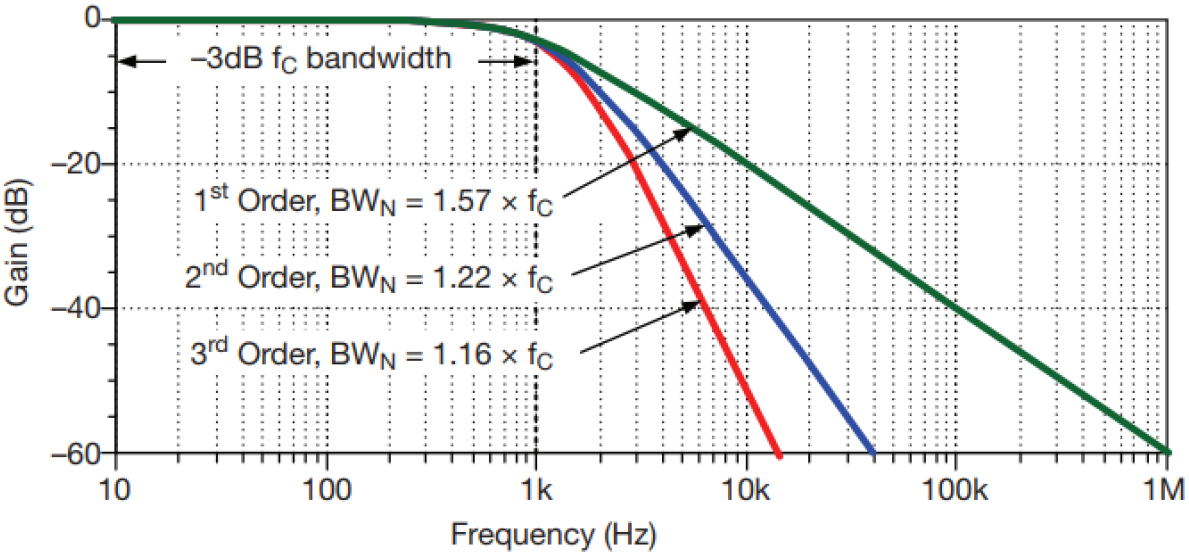
\includegraphics[width=\columnwidth]{images/rausch_bandbreite.png}
\end{minipage}
\hfill
\begin{minipage}[c]{0.38\columnwidth}
    \begin{tabular}{c | c}
        \toprule
        \textbf{Filterordnung}  & \textbf{ENB} \\
        \midrule
        $1$                     & $1.57 \cdot f_c$ \\
        \midrule
        $2$                     & $1.11 \cdot f_c$ \\
        \midrule
        $3$                     & $1.05 \cdot f_c$ \\
        \midrule
        $4$                     & $1.025 \cdot f_c$ \\
        \bottomrule
    \end{tabular}

\end{minipage}


\subsection{Rauschen von OpAmps}
\label{Rauschen von OpAmps}

\begin{minipage}[c]{0.4\columnwidth}
    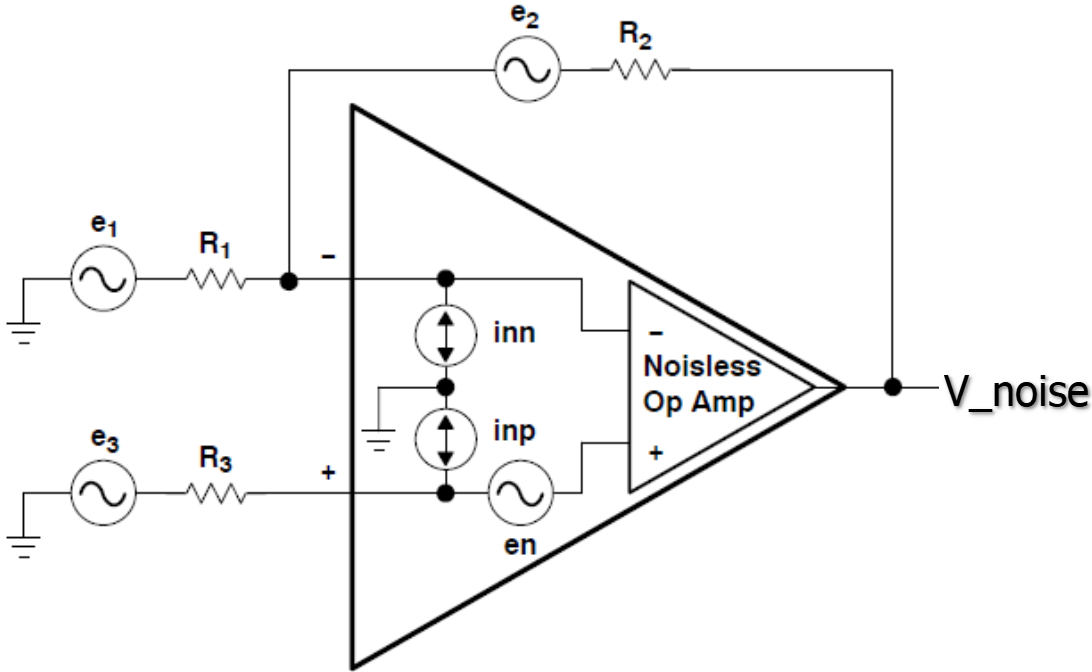
\includegraphics[width=\columnwidth]{images/rauschen_opamp.png}
\end{minipage}
\hfill
\begin{minipage}[c]{0.58\columnwidth}
    \begin{outline}
        \1 6 Rauschquellen 
            \2 $e_1$, $e_2$, $e_3$ sind \textbf{Rauschspannungen} der Widerstände
            \2 $e_n$ ist Rauschsppannungsdichte des OpAmps
            \2 $i_{nn}$, $i_{np}$ sind Eingangsströme des OpAmps
        \1 Ausgangsspannung $V_{\rm noise}$ wird berechnet mittels \textbf{Superposition}
    \end{outline}
\end{minipage}


Jede Quelle trägt folgendermassen zum gesamten Rauschen bei (exkl. Stromquellen):

\begin{minipage}[c]{0.4\columnwidth}
    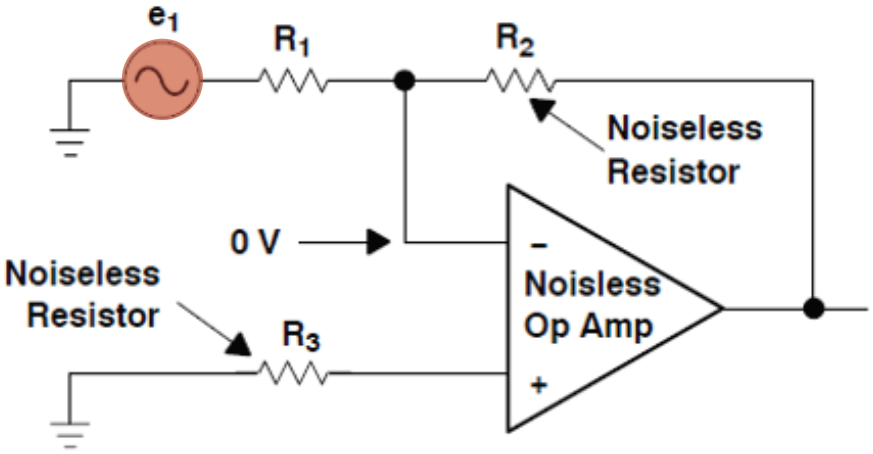
\includegraphics[width=\columnwidth]{images/rauschen_opamp_R1.png}
\end{minipage}
\hfill
\begin{minipage}[c]{0.4\columnwidth}
    Beitrag von $R_1$ wird \textbf{invertierend} verstärkt \\

    Rauschspannung: $ - \frac{R_2}{R_1} \cdot e_1$ \\
    Rauschleistung: $ \bigl(- \frac{R_2}{R_1} \bigr) \cdot e_1^2$
\end{minipage}


\begin{minipage}[c]{0.4\columnwidth}
    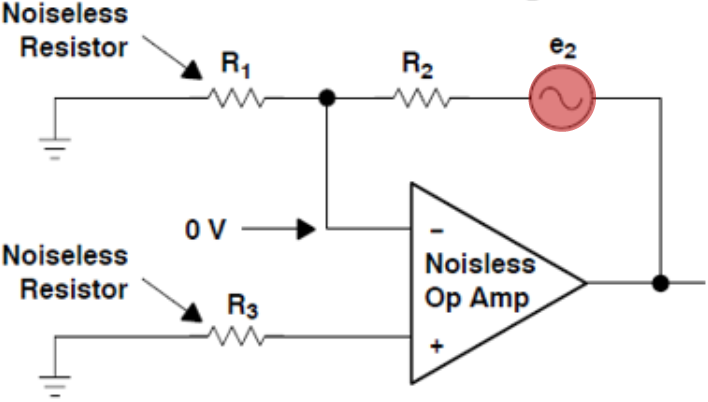
\includegraphics[width=\columnwidth]{images/rauschen_opamp_R2.png}
\end{minipage}
\hfill
\begin{minipage}[c]{0.4\columnwidth}
    Beitrag von $R_2$ wird \textbf{nicht} verstärkt \\

    Rauschspannung: $ 1 \cdot e_2$ \\
    Rauschleistung: $ 1 \cdot e_2^2$
\end{minipage}


\begin{minipage}[c]{0.4\columnwidth}
    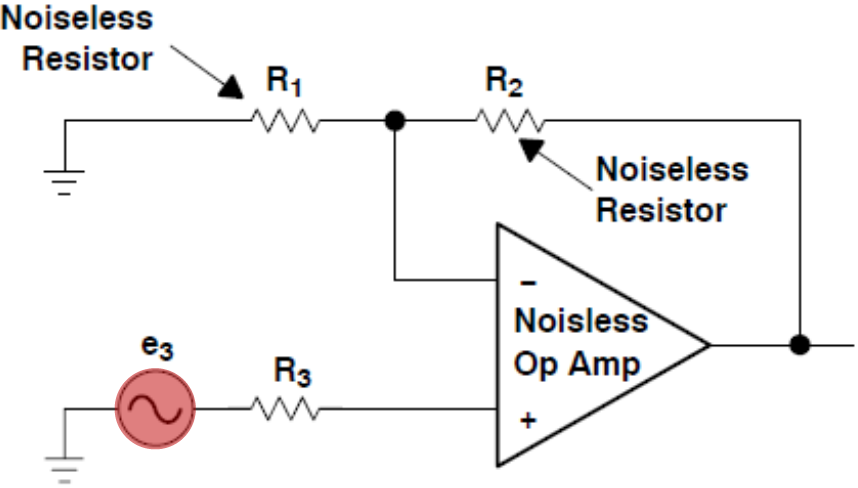
\includegraphics[width=\columnwidth]{images/rauschen_opamp_R3.png}
\end{minipage}
\hfill
\begin{minipage}[c]{0.4\columnwidth}
    Beitrag von $R_3$ wird \textbf{nicht-invertierend} verstärkt \\

    Rauschspannung: $ \frac{R_1 + R_2}{R_1} \cdot e_3$ \\
    Rauschleistung: $ \bigl(\frac{R_1 + R_2}{R_1} \bigr) \cdot e_3^2$
\end{minipage}


\begin{minipage}[c]{0.4\columnwidth}
    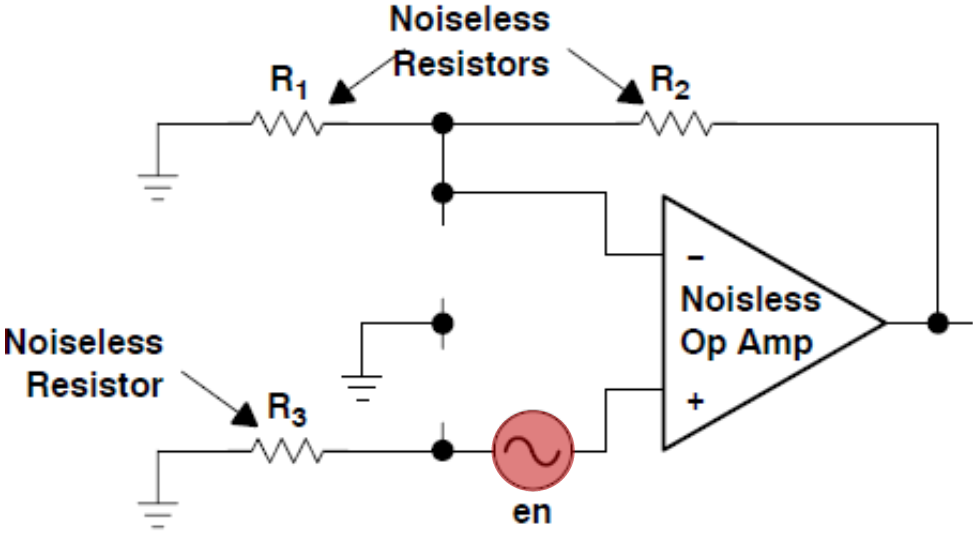
\includegraphics[width=\columnwidth]{images/rauschen_opamp_en.png}
\end{minipage}
\hfill
\begin{minipage}[c]{0.4\columnwidth}
    Beitrag von $e_n$ (OpAmp) wird \textbf{nicht-invertierend} verstärkt \\

    Rauschspannung: $ \frac{R_1 + R_2}{R_1} \cdot e_n$ \\
    Rauschleistung: $ \bigl(\frac{R_1 + R_2}{R_1} \bigr) \cdot e_n^2$
\end{minipage}

\vspace{0.2cm}
Für die \textbf{obige Beschaltung} (nicht allgemeingültig) ergibt sich somit gesamthaft:
$$ \boxed{ \scriptstyle{  V_{\rm noise} = \sqrt{ \int\limits_{0}^{\infty} \,  \Biggl[
    4 k T R_2 \Bigl( \frac{R_1 + R_2}{R_1} \Bigr)^2 + 4 k T R_3 \Bigl( \frac{R_1 + R_2}{R_1} \Bigr)^2
    + (i_{nn} R_2 )^2 + \Bigl(  i_{np} R_3 \Bigl( \frac{R_1 + R_2}{R_1} \Bigr) \Bigr)^2
    +  \Bigl(  e_n \Bigl( \frac{R_1 + R_2}{R_1} \Bigr) \Bigr)^2
    \Biggr] \, \diff f } }} $$

\textrightarrow\ Nicht vorhandene Elemente auf \textbf{Null} setzen!

\vspace{0.2cm}
\begin{minipage}[c]{0.48\columnwidth}
    \textbf{Hinweis:} Die meisten Elemente werden mit dem \textbf{Noise-Gain} $A_{\rm noise}$ multipliziert 
    (Verstärkung nicht-invertierender OpAmp)
\end{minipage}
\hfill
\begin{minipage}[c]{0.48\columnwidth}
    $$ \boxed{ A_{\rm noise} = \frac{R_1 + R_2}{R_1} = 1 + \frac{R_2}{R_1}}$$
\end{minipage}


\subsubsection{Vereinfachte Berechnung -- Rauschen von OpAmps}

Die vereinfachte Berechnung darf angewendet werden wenn: (UND-Verknüpfung)
\begin{itemize}
    \item Bandbreite $B \gg$ Noise Corner Frequency $f_{\rm enc}$ \\
        \textrightarrow\ Bandbreite $B > 10 \, \kilo \hertz$
    \item Widerstand $R_3 = 0$ (\textrightarrow\ Abschnitt~\ref{Rauschen von OpAmps})
\end{itemize}

$$ \boxed{ V_{\rm noise} = \sqrt{4 k T \cdot R_2 \cdot A_{\rm noise} \cdot \underbrace{ \frac{\pi}{2} \frac{\text{GBP}}{A_{\rm OPV}} }_{\text{ENB}}
+ e_w^2 \cdot A_{\rm noise}^2 \underbrace{ \frac{\pi}{2} \frac{\text{GBP}}{A_{\rm OPV}} }_{\text{ENB}} }} $$

\begin{tabular}{llc}
    ENB             & Effective Noise Bandwidth                 & $[\text{ENB}] = \hertz$ \\
    GBW             & Gain Bandwidth (Product)                  & $[\text{GWB}] = \hertz$ \\
    $A_{\rm noise}$ & Noise Gain                                & $[A_{\rm noise}] = 1$ \\
    $e_w$           & Rauschspannungsdichte (Datenblatt OpAmp)  & $[e_w] = \frac{\volt}{\sqrt{\hertz}}$ \\
\end{tabular}

\begin{tabular}{ll}
    $k$             & Boltzmann-Konstante $k = 1.38 \cdot 10^{-23} \, \frac{\joule}{\kelvin}$ \\
\end{tabular}
    
\textbf{Optimalfall:} Widerstände rauschen gleich viel wie OpAmp


\subsubsection{OpAmp Tiefpass -- Vereinfachte Berechnung}

\begin{minipage}[c]{0.35\columnwidth}
    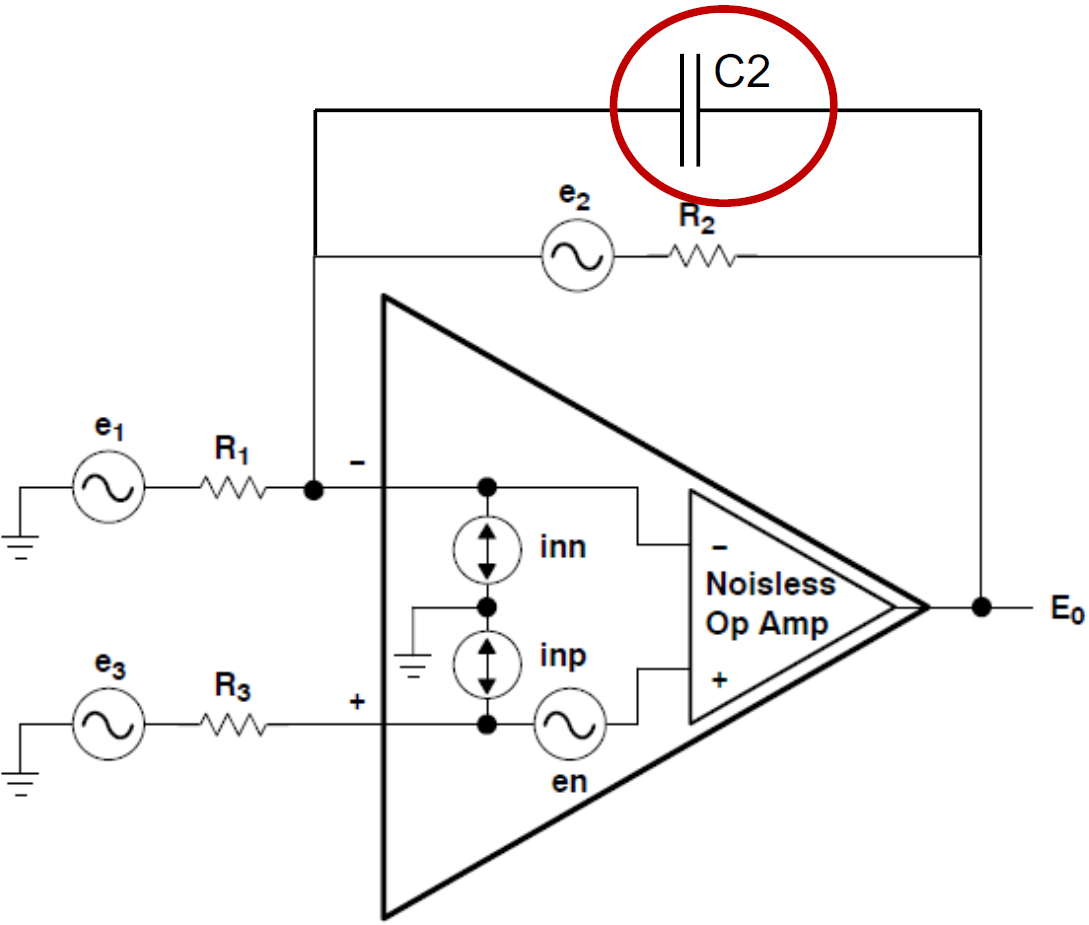
\includegraphics[width=\columnwidth]{images/rauschen_opamp_tiefpass.png}
\end{minipage}
\hfill
\begin{minipage}[c]{0.63\columnwidth}
    $$ \boxed{V_{\rm noise} = \sqrt{4 k T \cdot R_2 \cdot A_{\rm noise} \cdot \underbrace{ \frac{\pi}{2} f_{\rm TP}}_{\text{ENB}}
+ e_w^2 \cdot A_{\rm noise}^2 \underbrace{ \frac{\pi}{2} f_{\rm TP }}_{\text{ENB}} }} $$
$$ \text{mit } f_{\rm TP} = \frac{1}{2 \pi R_2 C_2} $$  % CHECK: stimmen Werte?
\end{minipage}


\subsubsection{Arten von Rauschen in OpAmps}

\begin{minipage}[c]{0.4\columnwidth}
    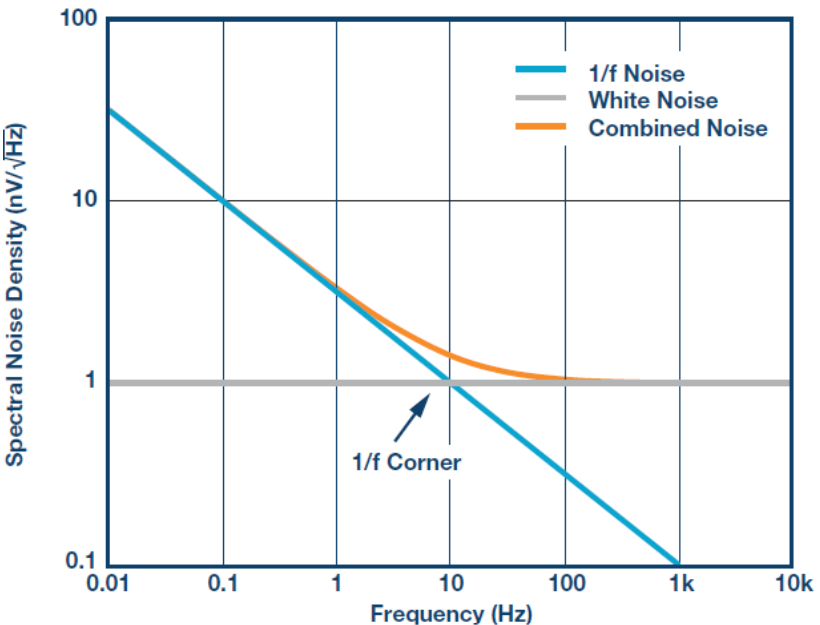
\includegraphics[width=\columnwidth]{images/rausch-arten_opamps.png}
\end{minipage}
\hfill
\begin{minipage}[c]{0.58\columnwidth}
    \raggedright
    \begin{outline}
        \1 Tiefe Frequenzen
            \2 Flicker-Noise ($\frac{1}{f}$-Rauschen) dominiert
        \1 Hohe Frequenzen
            \2 Weisses Rauschen dominiert
        \1 $\frac{1}{f}$-Corner \textrightarrow\ Noise-Corner-Frequency $f_{\rm enc}$
            \2 Weisses Rauschen gleich gross wie $\frac{1}{f}$-Rauschen
    \end{outline}
\end{minipage}


\subsection{Noise und Signal to Noise Ratio (SNR)}

\begin{minipage}[c]{0.48\columnwidth}
    $$ \boxed{ \text{SNR} = \frac{V_{\rm signal}}{V_{\rm rausch}} } $$
\end{minipage}
\hfill
\begin{minipage}[c]{0.48\columnwidth}
    $$ \boxed{ \text{SNR}_{\deci \bel} = 20 \cdot \log_{10} (\text{SNR})} $$
\end{minipage}


\example{Rauschen bei mehrstufigen Verstärkern}

\begin{minipage}[c]{0.4\columnwidth}
    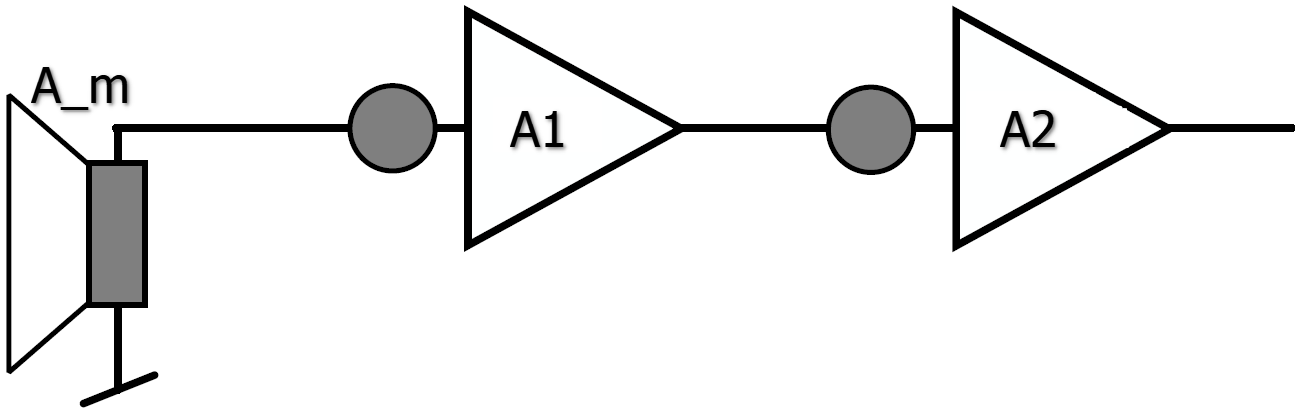
\includegraphics[width=\columnwidth]{images/signal_to_noise_ratio.png}
\end{minipage}
\hfill
\begin{minipage}[c]{0.58\columnwidth}
    Bei mehrstufigen Verstärkern sollten \textbf{grosse Verstärkungen möglist 'weit vorne'} in der Signalkette vorkommen.
\end{minipage}

$$ v_{n, \rm tot} = \sqrt{(v_{\rm mic} \cdot A_{\rm mic} \cdot A_1 \cdot A_2)^2
+ (v_{\rm OPV_1} \cdot A_1 \cdot A_2)^2 + (v_{\rm OPV_2} \cdot  A_2)^2 } $$


% könnte man auch weglassen
\subsection{Rauschen vermindern}

\begin{outline}
    \1 Weniger Rauschen $\Leftrightarrow$ mehr Strom
        \2 Gilt für Widerstände und aktive Bauteile
    \1 Bandbreite auf das Nötigste begrenzen
        \2 Tiefpass $> 1.$ Ordnung \textrightarrow\ ENB verkleinern
    \1 Verstärkung möglichst früh in Signalkette
    \1 Nicht-invertierender OpAmp besser als invertierender OpAmp
    \1 Verstärker parallel schalten
        \2 $n$-mal mehr Strom $\Leftrightarrow$ $\frac{1}{\sqrt{n}}$-mal weniger Rauschen
    \1 Differentielle Signale verwenden
        \2 Amplitude doppelt so gross
    \1 Referenzspannung filtern
    \1 Fignal HP-filtern \textrightarrow\ Reduktion $\frac{1}{f}$-Noise
    \1 Chopper- oder Sutozeroing-Verstärker \textrightarrow\ Reduktion $\frac{1}{f}$-Noise
    \1 Correlated Double Sampling (CDS)
    \1 Kühlen (teuer!)
\end{outline}